
%%%
% Any line that begins with a percent symbol is a comment. To compile
% this document and view the output:
%
% Run Latex
% Run Bibtex
% Then run Latex twice.
%
% This should produce the output PDF file named main.pdf
%%%

% This defines the style to use for this document.
% Do not modify.
\documentclass[letterpaper]{article}

% The following are akin to "import" statements in Python or Java -
% these import useful commands into the document for you to use.  You
% don't have to modify any of these lines. The AAAI package formats
% this document in the style of submissions to the American
% Association for Artificial Intelligence conference, one of the top
% AI conferences in the world. You will find that many academic
% publications in AI use this format.
\usepackage{aaai} 
\usepackage{times} 
\usepackage{helvet} 
\usepackage{courier} 
\setlength{\pdfpagewidth}{8.5in} 
\setlength{\pdfpageheight}{11in} 
\usepackage{amsmath}
\usepackage{amsthm}
\usepackage{graphicx}
\usepackage{graphics}
\usepackage{moreverb}
\usepackage{subfigure}
\usepackage{epsfig}
\usepackage{txfonts}
\usepackage{algpseudocode}
\usepackage{multirow, multicol}
\usepackage{url}
\usepackage{tablefootnote}
\usepackage{color}

\setcounter{secnumdepth}{1}
\nocopyright

% Fill in your paper title, names and emails below
% The "\\" is used to break lines. The \url command
% is useful for typesetting URLs and email addresses (it uses the
% Courier font).
\title{Solving Blackjack with Q-Learning}
 \author{Nathan Little \and Brad Shook\\
 \url{{nalittle, brshook}@davidson.edu}\\
 Davidson College\\
 Davidson, NC 28035\\
 U.S.A.}

% This is the "true" start of the document. All the text in your
% write-up should be placed within the \begin{document} and
% \end{document} decorators.
\begin{document}

\maketitle % formats the title nicely, do not modify

% While at this point you could just begin your write-up, often, it's
% useful to write each section of your write-up in a separate tex
% file (not unlike the modular decomposition you do for code you
% write). These \input commands insert the contents of the
% specified tex files in the order specified. Every write-up you
% submit must contain the following sections, in the shown order. Open
% each of the indicated tex files to understand what goes in each
% section, as well as for more TeX tips.

% Place the contents of your abstract between the
% \begin{abstract} and \end{abstract} decorators.

\begin{abstract}
In this paper, we build a Blackjack AI using Q-learning, a model-free reinforcement learning algorithm. We explore different parameter settings and assumptions, tuning the Q-learning algorithm for Blackjack. We subsequently evaluated the performance of our Q-learning bot against a random player and a heuristic player. While our bot did not converge to an optimal or near optimal policy, it did clearly outperform the random player. 

% The abstract should be between four and seven sentences long. Introduce the
% problem you are studying. Describe what you did. Summarize your results --- what
% did you discover, what is the main take-away message? Basically, you're trying 
% to sell your paper to the reader, so be brief and to the point. \textbf{Do \emph{not}
% include any citations in the abstract.}

% The \textbf{} command makes the specified text bold. The \emph{} or
% \textit{} command are used to italicize text. In general, text is never
% underlined.

% DON'T FORGET TO MATCH EACH OPEN BRACE WITH A CLOSING BRACE!
\end{abstract}



% The \section{} command formats and sets the title of this
% section. We'll deal with labels later.
\section{Introduction}
\label{sec:intro}
We designed an AI which learns and subsequently utilizes a policy for Blackjack. Our Blackjack AI uses the model-free reinforcement learning algorithm Q-learning in order to develop a policy with which to play the game. We set out to determine whether Q-learning would yield a policy which maximizes returns, and we evaluated the efficacy of our reinforcement learning approach against the results of two different Blackjack strategies: a random player and a heuristic player, which utilizes an optimal static policy. \\

\noindent The goal of our Q-learning algorithm was to derive an optimal policy which minimized losses or, more optimistically, maximized winnings. Blackjack is typically understood to hold a four percent disadvantage to the player who adheres to an optimal strategy, so such players should expect to lose \$4 for every \$100 bet \cite{b}. In their 1956 paper, Baldwin et al. devise an analytic approach to  Blackjack which yields a 0.62 percent disadvantage \cite{c}. Contemporary AI strategies often utilize Markov Chains since the game can be discretely modeled as a set of states, actions, transition probabilities and expected rewards, though such approaches often use card counting strategies to predict future states \cite{m}. At a high level, reinforcement learning algorithms are appealing to solve Blackjack since Blackjack is episodic and provides clear rewards in the form of winnings and losses. Indeed, de Granville finds that a Q-learning approach to Blackjack converges to a near optimal policy, outperforming the random player by a large margin \cite{q}. \\

\noindent In this paper, we will describe the Q-learning algorithm used by our player, summarize the details of our experiments, and then evaluate the performance of our player against other strategies. 


% In this section, you should introduce the reader to the problem you
% are attempting to solve. For example, for the first project: describe
% the dataset, and the prediction problem that you are
% investigating. You should also cite and briefly describe other related
% papers that have tackled this problem (or similar ones) in the past
% --- things that came up during the course of your research. In the
% AAAI style, citations look like \cite{aima} (see
% the comments in the source file \texttt{intro.tex} to see how this
% citation was produced). Conclude by summarizing how the
% remainder of the paper is organized. \\

% Citations: As you can see above, you create a citation by using the
% \cite{} command. Inside the braces, you provide a "key" that is
% uniue to the paper/book/resource you are citing. How do you
% associate a key with a specific paper? You do so in a separate bib
% file --- for this document, the bib file is called
% project1.bib. Open that file to continue reading...

% Note that merely hitting the "return" key will not start a new line
% in LaTeX. To break a line, you need to end it with \\. To begin a 
% new paragraph, end a line with \\, leave a blank
% line, and then start the next line (like in this example).
% Overall, the aim in this section is context-setting: what is the
% big-picture surrounding the problem you are tackling here?



\section{Background}
\label{sec:background}

\subsection{Blackjack Domain}

The objective of Blackjack is to obtain a higher number of points than the dealer without exceeding 21, where points are determined by cards held. Cards numbered 2 through 10 are worth their face value; face cards (Jack, Queen, King) are worth 10 points each; and aces are worth either 1 or 11 points. Our game consists of one player, the dealer, and one 52-card deck, shuffled prior to each game. The player bets \$1 prior to each hand, and the player and dealer are dealt two cards each, where only the value of the dealer's first card is known to the player. The player can then choose to either hit, which entails being dealt an additional card, or stand with the current hand, ending the player's turn. If the player exceeds 21, the game is over and the dealer wins the player's \$1. If not, the dealer hits until her points reach 17 or greater, in which case she must stand. \\

\noindent Blackjack players evaluate their hand relative to the dealer's card, often assuming that the dealer's hidden card is of value 10 \cite{b}. Since cards of value 10 account for 30 percent of cards in a 52 card deck, a plurality, they are the most likely point value for the dealer to hold. Such an assumption gives an approximate upper bound for the dealer's point total and is therefore a useful assumption to roughly estimate the actual state of the game. For instance, typical Blackjack wisdom holds that players ought to stand if the dealer shows a 6 and the player has some point total above 11. Since the dealer is likely to have 16 total points, she is likely to bust once she hits (which the dealer must do at sixteen). We explore the impact of the 10 point assumption in this paper. 

% 30 percent of cards in a 52-card deck are of point value 10, so we assume that the dealer's hidden card is always of value ten. This approach, therefore, represents the worst case scenario for  


% Since the dealer's second card is unknown to the player, she assumes that the dealer's points are their first card's value plus ten .

% (MAYBE THIS SHOULD GO IN Q LEARNING SINCE IT IS UNIQUE TO THAT????? - not really unique to Q learning but a relatively typical way to think about blackjack). Actually, I think maybe it should go in Q-learning since its not a proper part of the game but rather an assumption our player uses. 




% Describe any background information that the reader would need to know
% to understand your work. You do not have to explain algorithms or
% ideas that we have seen in class. Rather, use this section to describe
% techniques that you found elsewhere in the course of your research,
% that you have decided to bring to bear on the problem at hand. Don't
% go overboard here --- if what you're doing is quite detailed, it's
% often more helpful to give a sketch of the big ideas of the approaches
% that you will be using. You can then say something like ``the reader
% is referred to X for a more in-depth description of...'', and include
% a citation.\\

% This section is also a good place to describe any data pre-processing
% or feature engineering you may have performed. If you are \emph{only}
% discussing data wrangling in this section, it's recommended that you
% amend the title of the section to ``Data Preparation'' or something
% similar; otherwise, use subsections to better organize the flow.

\subsection{Q-Learning}
Q-learning is a model-free reinforcement learning algorithm. More specifically, Q-learning is a temporal difference algorithm which directly approximates the optimal state-action value function $Q^* (s,a)$, which is defined as the expected sum of discounted future rewards assuming that the agent takes action $a$ in state $s$, acting optimally in each later state \cite{rn}. The optimal state-action value function is obtained by updating the state-action value function $Q(s,a)$ episodically, so in Blackjack, $Q(s,a)$ is updated after each game. The optimal policy is that which maximizes rewards over time. De Granville provides the following pseudocode for the Q-learning algorithm: \\ 

    \noindent Initialize $Q(s,a)$ arbitrarily \\
    
    \noindent For each episode: \
    
        Choose $a$ from $s$ using policy derived from $Q$ \
        
        Take action $a$, observe reward $r$, and new state $s'$ \
        
        $Q(s,a) = Q(s,a) + \alpha[r + \gamma \text{ max}_{a'} Q(s',a') - Q(s,a)]$ \
        
        $s = s'$ \
        
    \noindent until $s$ is terminal \\

\noindent Note that $\alpha$ refers to the learning rate, which determines the size of the update made each episode, and $\gamma$ is the discount rate, which determines the weight of future rewards \cite{q}. For selecting an action to take from a given state, many Q-learning algorithms use the epsilon-greedy strategy. This strategy introduces randomness to the selection of actions which allows the algorithm to better train the policies and avoid local minima. \\

\noindent If each state-action pair is continually updated, Q-learning is expected to converge to the optimal state-action value function with probability 1 \cite{q}. Because Q-learning begins with an arbitrary model, it is expected to perform similarly to the random player at first. It should subsequently tend towards the performance of the heuristic player as it learns, developing a policy which approaches optimality. 


\subsection{Other Policies}
In order to evaluate the success of our Q-learning algorithm, we compare its results to that of a random player and a heuristic player, which utilizes a basic, static policy. 

\begin{itemize}
    \item \textbf{Random Player}: randomly chooses an action, either hit or stand, at each given state where each action has an equal probability of being chosen. 
    \item \textbf{Heuristic Player}: leverages a near-optimal static policy proposed by Howard \cite{o}. The policy is given by the following set of rules: \ 
    
    \begin{figure}[htb]
      \centering  % centers the image in the column
      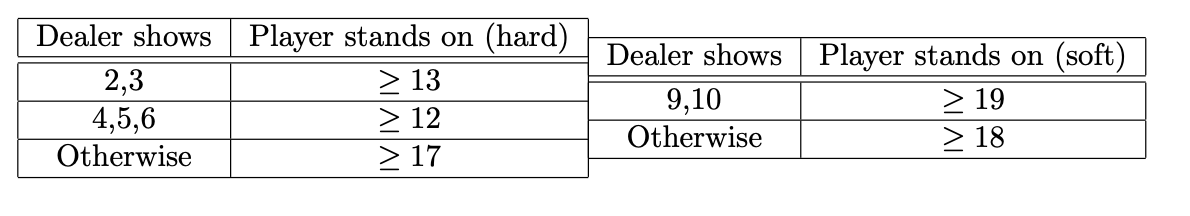
\includegraphics[width = 3.4in]{a.png} 
      % *Every* figure should have a descriptive caption.
      \caption{Static Blackjack policy. Image courtesy of \texttt{Howard $2016$}.}
     \label{fig:tex}

    \end{figure}
\end{itemize}
\noindent We call the heuristic policy static since the player adheres to the strict set of rules in order to make decisions at each given state. A typical optimal policy gives the player a 4 percent disadvantage, so we consider this policy near optimal. \\

\noindent The random and heuristic players set realistic lower and upper bounds, respectively, on the performance of our player. Our goal for the Q-learning algorithm was to devise a policy which tends towards, and ideally would exceed, the performance of the heuristic policy. 





\section{Experiments}
\label{sec:expts}
In order to determine the efficacy of our Q-learning Blackjack player, we experimented with different parameter settings, testing each on 100,000 hands, and compared the results of 100,000 hands played by the Q-learning bot, the random bot, and the heuristic bot. Prior to playing the 100,000 round game, the Q-learning bot was trained on 1,000,000 hands. The lone deck was shuffled prior to each hand played, and each game consisted only of the dealer and a single player. 

\subsection{Experiment 1: Parameter Settings}
In Experiment 1, we attempted to determine how two parameters, alpha and gamma, affected the performance of the Q-learning bot in terms of average rewards. The effects of alpha, the learning rate, were found by training 9 Q-learning policies, each with a different alpha value ranging from 0.1 to 0.9. Each of these policies had a gamma of 0.9 and an epsilon value of 0.1. Moreover, the effects of gamma, the discount factor, were derived by training 9 additional Q-learning policies, each with a different gamma ranging from 0.1 to 0.9. Each gamma test had alpha and epsilon values of 0.1. Each of these aforementioned policies were trained for 1,000,000 episodes. After training, 100,000 matches of Blackjack were played with each policy and the win differential was updated after each game. This experiment allowed us to determined if there were optimal values for these two parameters. 

\subsection{Experiment 2: Player Performance}
The goal of Experiment 2 was to evaluate the performance of the Q-learning bot relative to the random bot and the heuristic bot. First, the Q-learning bot was given a set of parameters (.1 for epsilon, .1 for alpha, and .9 for gamma) and trained on 1,000,000 hands. Then, each bot played 100,000 hands of Blackjack. The average reward was updated after each match, and we used these reward averages to determine the varying performance among the bots. We also experimented with the assumption that the dealer's hidden card is a 10, again running 100,000 hands for policies trained with and without that assumption. 

% In this section, you should describe your experimental setup. What
% were the questions you were trying to answer? What was the
% experimental setup (number of trials, parameter settings, etc.)? What
% were you measuring? You should justify these choices when
% necessary. The accepted wisdom is that there should be enough detail
% in this section that I could reproduce your work \emph{exactly} if I
% were so motivated.


\section{Results}
\label{sec:results}

% Present the results of your experiments. Simply presenting the data is
% insufficient! You need to analyze your results. What did you discover?
% What is interesting about your results? Were the results what you
% expected? Use appropriate visualizations. Prefer graphs and charts to
% tables as they are easier to read (though tables are often more
% compact, and can be a better choice if you're squeezed for space).


\subsection{Results of Experiment 1: Parameter Settings}
\label{sec:resE1}
Since we had a limited number of future states in each game, the first and last states in a game were close to each other. Thus, changes in gamma minimally impacted the performance of the Q-learning bot. Since our algorithm was not particularly expensive in terms of either space or time complexity, we were able to train our policy on a large number of hands. Thus, alpha had minimal impact on the performance of our algorithm because we trained the policy on 1,000,000 hands. The lack of correlation between the alpha and gamma settings with average rewards is shown in Figure \ref{hpFig}. This graph shows that these parameters had little to no effect on the average rewards of the Q-learning bot. 

\begin{figure}[htb]

  \centering  % centers the image in the column

  % replace the second argument below with your filename. I like to
  % place all my figures in a sub-directory to keep things organized
  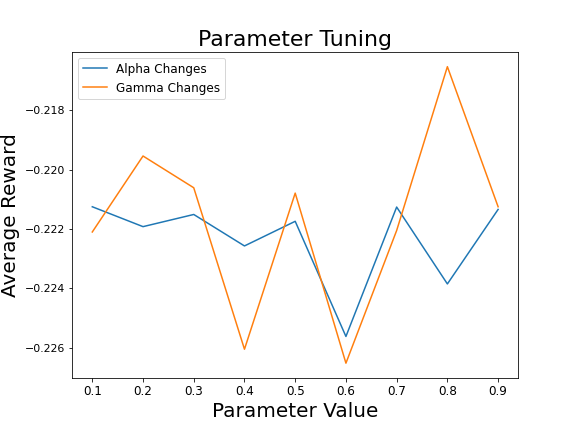
\includegraphics[width=0.47\textwidth]{hpTuning.png}


  % *Every* figure should have a descriptive caption.
  \caption{Comparison of average rewards for policies trained with varying alpha and gamma values.}

  \label{hpFig}

\end{figure}

\subsection{Results of Experiment 2: Player Performance}
\label{sec:resE2}
As shown in Figure \ref{avgRewards}, our bot quickly outperformed the random player, reaching higher average rewards after only a few thousand hands. Subsequently, our bot failed to improve its performance, however. Figure \ref{avgRewards} shows the Q-learning bot's early plateau: failing to improve at all after about 20,000 hands. In our experiment, the Q-learning bot failed to converge to an optimal policy or anything remotely close to optimal. Our bot averaged a reward of $-22$ percent whereas an optimal policy should make returns close to $-4$ percent. The random bot realized approximately $-25$ percent returns, just 3 percentage points worse than our player. These results suggest that our Q-learning bot was not able to effectively learn optimal policies that mirrored those used in the heuristic bot.\\

\noindent Furthermore, the assumption that the dealer's hidden card is of value 10 proved to have no impact on the performance of our player. We experimented with and without the assumption on different parameter settings, but the Q-learning bot realized average returns which were 99 percent similar, both converging to approximately $-22$ percent. 

\begin{figure}[htb]

  \centering  % centers the image in the column

  % replace the second argument below with your filename. I like to
  % place all my figures in a sub-directory to keep things organized
  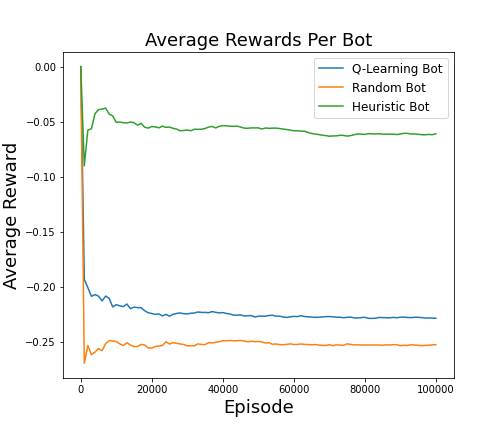
\includegraphics[width=0.47\textwidth]{avgRewardsPerBot.png}


  % *Every* figure should have a descriptive caption.
  \caption{Comparison of average rewards for the Q-learning bot, random bot, and heuristic bot.}

  \label{avgRewards}

\end{figure}





\section{Conclusions}
\label{sec:concl}
We set out to study the performance of a Q-learning algorithm applied to Blackjack. We determined that while Q-learning outperforms a random player, it failed to converge to an optimal strategy, which contradicts the results of de Granville. This result could be due to the fact that de Granville also used actions such as double-down, insurance, and splitting a hand, each of which allow for higher average returns in certain scenarios. In the future, we would expand our algorithm to include these additional actions. We might also define states more specifically, using the actual cards held instead of just the point value of the hand. This would provide our bot more information concerning the current state of the game, thus informing decision making. 

% In this section, briefly summarize your paper --- what problem did you
% start out to study, and what did you find? What is the key result /
% take-away message? It's also traditional to suggest one or two avenues
% for further work, but this is optional.

% Adding more actions, incorporate card counting, higher degree of randomness since we hit a plateau. Expand states in terms of cards held, not just the total point value. 

\section{Contributions}
\label{sec:contrib}
BS and NL contributed equally to the project. We did almost all of the coding collaboratively over VS Code LiveShare. On the paper, NL primarily focused on the Introduction and Background while BS spent more time on the Experiments and Results sections. That said, both BS and NL worked on every section of the paper. Both NL and BS collected data for the paper, but BS, in particular, collected most data and made the graphs. 

% Briefly summarize the contributions of you and your partner in this
% section. For example: ``A.T. wrote the gradient descent code and ran
% experiments; J.vN. ran the experiments using scikit-learn's built-in
% regression solver. A.T. wrote the introduction and background sections
% and prepared figure \ref{fig:tex} and table
% \ref{tab:example}. J.vN. wrote the experiments and results
% sections. Both authors proof-read the entire document.'' I will be
% looking for roughly equal contributions from both partners in both
% aspects of the assignment (i.e., the programming/data
% preprocessing/experimentation and writing).



\section{Acknowledgements} 
\label{sec:ack} 
We would like to thank Dr. Raghu Ramanujan for his insight and guidance throughout the process.
% This section is optional. But if there are people you'd like to thank for their help with the project --- a person who contributed some insight, friends who volunteered to help out with data collection, etc. --- then this is the place to thank them. Keep it short!


% This creates the references section. Open the project1.bib file to
% see how to organize your references.
\bibliography{project1}
\bibliographystyle{aaai} % sets citation and bib style, do not modify

\end{document}
